% Generated by book/tools/notebook_to_tex.py. Do not edit by hand.

\chapter[작은 BERT 이진 분류 (NSMC)]{작은 BERT 이진 분류 (Korean NSMC Fine-tuning)}

\label{ch:23}

\markboth{작은 BERT 이진 분류 (NSMC)}{작은 BERT 이진 분류 (NSMC)}

\chaptermeta{23_ko_bert_classify/23_ko_bert_classify.ipynb}{https://colab.research.google.com/github/yoon-gu/neuqes-101/blob/master/23_ko_bert_classify/23_ko_bert_classify.ipynb}{22장에서 사전학습한 한국어 작은 BERT 본체를 NSMC 이진 분류로 파인튜닝}



\index{1Korean BERT fine tuning@Korean BERT fine-tuning}

\index{1BertForSequenceClassification@BertForSequenceClassification}

\index{1NSMC@NSMC}

\index{1binary classification@binary classification}

\index{1CrossEntropyLoss@CrossEntropyLoss}

\index{1classification head@classification head}

\index{1transfer learning@transfer learning}

\index{1KLUE BERT comparison@KLUE-BERT comparison}

\index{1confusion matrix@confusion\_matrix}

\index{1classification report@classification\_report}

\index{1roc auc score@roc\_auc\_score}

\index{0한국어 이진 분류@한국어 이진 분류}

\index{0파인튜닝@파인튜닝}

\index{0전이 학습@전이 학습}

\index{0분류 헤드@분류 헤드}

\index{0혼동 행렬@혼동 행렬}

\index{1load state dict@load\_state\_dict}

\index{1classifier head@classifier head}

\index{1single label classification@single\_label\_classification}

\index{1softmax@softmax}

\index{1fine tune loss@fine-tune loss}

\index{1NSMC binary classification@NSMC binary classification}

\index{1domain transfer@domain transfer}

\index{1random baseline@random baseline}

\index{1head replacement@head replacement}

\index{1body weight transfer@body weight transfer}

\index{1negative transfer@negative transfer}

\index{0본체 가중치@본체 가중치}

\index{0헤드 교체@헤드 교체}

\index{0도메인 전이@도메인 전이}

\index{0한국어 분류@한국어 분류}

\index{0태스크 도메인@태스크 도메인}

\index{0정확도@정확도}

\index{1AUC@AUC}



\section{변화추적표}

\begin{booktable}{23장 변화추적표}{tab:ch23-01}
\begin{adjustbox}{max width=\textwidth}
\begin{tabular}{@{}lllllll@{}}
\toprule
Ch & 모델 & 토크나이저 & 데이터 & Output Head & Activation & Loss \\
\midrule

15 & \inlinecode{klue/bert-base} 파인튜닝 (약 110M) & WordPiece (한국어, 사전학습) & NSMC (네이버 영화 리뷰, 이진) & \inlinecode{Linear(H,\ 2)} & softmax & \inlinecode{CrossEntropyLoss} \\
20 & 작은 BERT (직접, scratch) & \inlinecode{bert-base-uncased} 토크나이저 (가져옴) & Wikitext-103 paragraphs (일반 도메인) & MLM head & softmax (MLM) & \inlinecode{CrossEntropyLoss} (masked token) \\
21 & \ref{ch:20}장 사전학습 BERT + 분류 헤드 (약 10M) & (\ref{ch:20}장과 동일) & Yelp 이진화 (다른 도메인 transfer) & \inlinecode{Linear(H,\ 2)} & softmax & \inlinecode{CrossEntropyLoss} \\
22 & 작은 BERT (직접, scratch) --- 한국어 & \inlinecode{klue/bert-base} 토크나이저 (가져옴) & 한국어 Wikipedia paragraphs (일반 도메인) & MLM head & softmax (MLM) & \inlinecode{CrossEntropyLoss} (masked token) \\
\textbf{23 \(\leftarrow\) 여기} & \textbf{\ref{ch:22}장 사전학습 BERT + 분류 헤드 (약 10M)} & \textbf{(\ref{ch:22}장과 동일)} & \textbf{NSMC 이진 (다른 도메인 transfer)} & \textbf{\inlinecode{Linear(H,\ 2)}} & \textbf{softmax} & \textbf{\inlinecode{CrossEntropyLoss}} \\
24 (다음, Phase 4) & GPT-2 (직접, scratch) & BPE 토크나이저 (직접 학습) & TinyStories 영어 동화 & LM head & softmax (next-token) & \inlinecode{CrossEntropyLoss} (causal LM) \\
\bottomrule
\end{tabular}
\end{adjustbox}
\end{booktable}

전체 장 표는 \href{https://github.com/yoon-gu/neuqes-101\#챕터별-변화추적표}{루트 README.md}를 참고하세요.

\textbf{Phase 3 안에서의 위치} --- \ref{ch:19}장 (토크나이저 학습) \(\to\) \ref{ch:20}장 (영어 모델 사전학습) \(\to\) \ref{ch:21}장 (영어 분류) \(\to\) \ref{ch:22}장 (한국어 모델 사전학습) \(\to\) \textbf{\ref{ch:23}장 (한국어 분류, Phase 3 종료)}. \ref{ch:22}장 \(\to\) \ref{ch:23}장 흐름이 \ref{ch:20}장 \(\to\) \ref{ch:21}장 흐름의 \emph{한국어 대칭본}. 본문의 클라이맥스는 \emph{2-way 비교} --- \ref{ch:15}장의 대규모 사전학습 모델과 본 장의 작은 자체 사전학습 모델의 격차로 \emph{사전학습 규모의 가치} 를 정량 측정. 사전학습 자체의 \emph{순} 효과 (random init baseline 대비) 와 \emph{한국어 환경 특유의 negative transfer 가능성} 은 부록에서 다룹니다.



\section{변경점: \ref{ch:22}장 대비}

\begin{booktable}{23장 변경점 요약}{tab:ch23-02}
\begin{adjustbox}{max width=\textwidth}
\begin{tabular}{@{}lll@{}}
\toprule
축 & \ref{ch:22}장 (한국어 MLM scratch) & \ref{ch:23}장 (한국어 분류 fine-tune) \\
\midrule

\textbf{이 장의 task} & MLM 사전학습 (masked token 예측) & \textbf{이진 분류 (NSMC 긍정/부정)} \(\leftarrow\) \emph{task 축 변화} \\
모델 클래스 & \inlinecode{BertForMaskedLM} & \textbf{\inlinecode{BertForSequenceClassification(num\_labels=2)}} \\
본체 (embedding + encoder) & random init \(\to\) 한국어 위키 MLM 학습 & \textbf{\ref{ch:22}장 사전학습 본체 그대로 이어받음} \\
출력 헤드 & MLM head (vocab 약 32,000 차원) & \textbf{분류 head (\inlinecode{Linear(256,\ 2)})} \(\leftarrow\) 새 random init \\
토크나이저 & \inlinecode{klue/bert-base} (vocab 약 32,000) & (그대로) \\
\textbf{데이터} & \textbf{한국어 Wikipedia paragraphs (일반 도메인, 라벨 없음)} & \textbf{NSMC 영화 리뷰 (다른 도메인, 라벨 사용)} \(\leftarrow\) \emph{사전학습과 fine-tune 도메인이 다름} \\
Loss & \inlinecode{CrossEntropyLoss} (vocab 약 32,000 logits) & \textbf{\inlinecode{CrossEntropyLoss} (2 logits)} \(\leftarrow\) K 만 큰 변화 \\
학습률 & 5e-4 (scratch MLM) & \textbf{2e-5} (fine-tune 표준) \\
\bottomrule
\end{tabular}
\end{adjustbox}
\end{booktable}

\begin{quote}
\textbf{변경점 한 가지 원칙} --- Phase 3 안에서 \emph{task 축} 이 변합니다 (MLM \(\to\) 분류). 데이터 \emph{도메인} 도 같이 변합니다 (위키 \(\to\) NSMC) --- 이게 \emph{진짜 transfer 의 본질}. 모델 본체·토크나이저는 그대로, 헤드와 라벨 형식·데이터 도메인이 바뀝니다. 이게 \emph{사전학습-fine-tune 패러다임} 의 핵심: 본체는 한 번 학습한 \emph{일반 표상} 을 재사용, downstream task 도메인마다 \emph{작은 헤드 + 작은 학습률} 로 적응.
\end{quote}

\subsection{두 데이터셋의 역할}

본 장의 특수성 --- 한 노트북에 두 데이터셋이 함께 들어갑니다.

\begin{booktable}{23장 두 데이터셋의 역할 표}{tab:ch23-03}
\begin{adjustbox}{max width=\textwidth}
\begin{tabular}{@{}lll@{}}
\toprule
단계 & 데이터셋 & 용도 \\
\midrule

3 §MLM 사전학습 & \inlinecode{wikimedia/wikipedia}, \inlinecode{20231101.ko} 2K paragraphs \(\times\) 3 epoch & self-supervised MLM (라벨 없음, 일반 위키 본문) \\
4-5 §분류 fine-tune & NSMC (e9t/nsmc GitHub raw TSV) 5K/1K & supervised 이진 분류 (긍정/부정 라벨) \\
\bottomrule
\end{tabular}
\end{adjustbox}
\end{booktable}

같은 토크나이저 (\inlinecode{klue/bert-base}) 가 두 데이터셋의 모든 텍스트를 처리. 본체가 \emph{일반 위키 어휘} 로 사전학습된 표상이 \emph{영화 리뷰 비격식 구어체 토큰} 에 얼마나 잘 전이되는가가 본 장의 측정 대상.

\subsection{\texorpdfstring{\ref{ch:15}장 (klue/bert-base) 와의 비교가 본 장의 메인 메시지 --- 이제 \emph{fair}}{\ref{ch:15}장 (klue/bert-base) 와의 비교가 본 장의 메인 메시지 --- 이제 fair}}

\begin{booktable}{23장 15장 (klue/bert-base) 와의 비교가 본 장의 메인 메시지 - 이제 fair 표}{tab:ch23-04}
\begin{adjustbox}{max width=\textwidth}
\begin{tabular}{@{}llll@{}}
\toprule
차원 & \ref{ch:15}장 (klue/bert-base) & \ref{ch:23}장 (이 장) & 비고 \\
\midrule

본체 파라미터 & 약 110M & \textbf{약 10M} & \ref{ch:23}장 은 1/11 작음 \\
사전학습 코퍼스 & 한국어 위키 + 모두의 말뭉치 + 뉴스 + 댓글 (약 8.4B 토큰, 일반 도메인) & \textbf{한국어 Wikipedia paragraphs 5K (약 50만-80만 토큰, 일반 도메인)} & 약 10,000배 격차, \textbf{둘 다 일반 한국어 코퍼스} \\
사전학습 시간 & TPU 수일 & \textbf{T4 약 8-10분} & \\
Fine-tune 도메인 & NSMC 이진 (사전학습과 다른 도메인) & NSMC 이진 (사전학습과 다른 도메인) & \textbf{둘 다 일반 한국어 \(\to\) NSMC transfer 라 fair} \\
분류 fine-tune 셋업 & \ref{ch:15}장 = 이 장 동일 (같은 데이터, 같은 hyperparams) & & 변하는 건 \emph{본체 출발점} 뿐 \\
실측 accuracy & 약 0.86 & \textbf{약 0.54} & 실행본 기준 (\ref{ch:15}장=0.86, \ref{ch:23}장=0.5420). 짧은 사전학습(MLM 약 0.2분)이라 동전 던지기에 가까움 \\
\bottomrule
\end{tabular}
\end{adjustbox}
\end{booktable}

비교가 \emph{공정} 한 이유 --- \ref{ch:15}장도 본 장도 둘 다 \emph{일반 도메인 한국어 사전학습 \(\to\) NSMC 분류 transfer} 의 같은 패턴. \emph{사전학습 규모} (약 10,000배) 와 \emph{모델 크기} (11배) 만 차이. 만약 \ref{ch:23}장 이 NSMC text 로 사전학습했다면 비교가 unfair 했을 것 --- domain-adaptive pretraining 우위 때문.

\subsection{\texorpdfstring{\ref{ch:21}장 (영어) \(\to\) \ref{ch:23}장 (한국어) 대칭}{\ref{ch:21}장 (영어) \textbackslash to \ref{ch:23}장 (한국어) 대칭}}

\begin{booktable}{23장 21장 (영어) \textbackslash to 23장 (한국어) 대칭 표}{tab:ch23-05}
\begin{adjustbox}{max width=\textwidth}
\begin{tabular}{@{}lll@{}}
\toprule
항목 & \ref{ch:21}장 (영어) & \ref{ch:23}장 (한국어, 이 장) \\
\midrule

사전학습 코퍼스 (일반 도메인) & Wikitext-103 paragraphs 5K & 한국어 Wikipedia paragraphs 5K \\
분류 데이터 (다른 도메인) & Yelp polarity 5K/1K & NSMC 5K/1K \\
비교 대상 (대규모 사전학습) & \ref{ch:10}장 (DistilBERT, 약 66M, 약 33억 토큰) & \ref{ch:15}장 (\inlinecode{klue/bert-base}, 약 110M, 약 8.4B 토큰) \\
토크나이저 & \inlinecode{bert-base-uncased} & \inlinecode{klue/bert-base} \\
메시지 & \emph{일반 위키 사전학습 \(\to\) 영화 리뷰 transfer} & \emph{일반 위키 사전학습 \(\to\) 영화 리뷰 transfer} \\
\bottomrule
\end{tabular}
\end{adjustbox}
\end{booktable}

같은 결을 한국어 환경에서 재확인 --- Phase 3 의 마지막 검증.



\section{\texorpdfstring{손실 함수의 변화: MLM에서 분류 CE로}{Loss 함수의 변화 --- MLM CE (vocab 약 32,000) \textbackslash to 분류 CE (K=2)}}

\ref{ch:22}장의 MLM 도 본질은 \emph{vocab 위에서의 다중 분류} 였습니다. 다만 K = vocab\_size 약 32,000 이라 어려운 task. 이 장는 K = 2 의 \emph{훨씬 쉬운} 분류 task.

\subsection{수식}

분류 task 의 CE 는 \ref{ch:15}장 / \ref{ch:21}장과 같습니다 (K=2):

\begin{equation}
\label{eq:ch23-01}
L_{\text{cls}} = -\frac{1}{N}\sum_{i=1}^{N} \log \hat p_{i, y_i}
\end{equation}

식~\eqref{eq:ch23-01}은 이 절에서 사용하는 핵심 관계를 정리한 것입니다.

\begin{itemize}
\tightlist
\item
  \(\hat p_{i, k} = \mathrm{softmax}(z_i)_k\) --- K=2 차원 softmax
\item
  \(y_i \in \{0, 1\}\) --- 정수 라벨 (NSMC: 0=negative, 1=positive)
\end{itemize}

\subsection{두 CE 기준선 비교}

\begin{booktable}{23장 두 CE 기준선 비교 표}{tab:ch23-06}
\begin{adjustbox}{max width=\textwidth}
\begin{tabular}{@{}llll@{}}
\toprule
task & K & random baseline loss \(\log K\) & 학습 어려움 \\
\midrule

MLM (\ref{ch:22}장) & 약 32,000 & \textbf{10.37} & 매우 어려움 --- 가려진 토큰 자리에 \emph{vocab 전체 후보} 중 정답을 \\
분류 (\ref{ch:23}장) & 2 & \textbf{0.693} & 상대적으로 쉬움 --- 긍정/부정 둘 중 하나 \\
\bottomrule
\end{tabular}
\end{adjustbox}
\end{booktable}

학습 첫 step 의 loss 가 약 0.693 부근이면 모델이 \emph{균등 추측} 단계. fine-tune 첫 step 에서 분류 헤드만 새로 init 됐으므로 \emph{이 정도} 가 정상.

\subsection{\texorpdfstring{사전학습 효과와 loss 곡선}{사전학습 효과가 loss 곡선 에 어떻게 드러나나}}

\begin{booktable}{23장 사전학습 효과가 loss 곡선 에 어떻게 드러나나 표}{tab:ch23-07}
\begin{adjustbox}{max width=\textwidth}
\begin{tabular}{@{}llll@{}}
\toprule
셋업 & 학습 첫 step loss & 학습 종료 loss (epoch 2) & 메모 \\
\midrule

한국어 Wikipedia MLM 사전학습 본체 + 분류 (본 장) & 약 0.693 & \textbf{약 0.45-0.6} & 본체에 \emph{일반 한국어 어휘·문맥 구조} 가 들어 있어 헤드가 NSMC 분류로 비교적 빠르게 적응 \\
\ref{ch:15}장 \inlinecode{klue/bert-base} 사전학습 본체 + 분류 & 약 0.693 & \textbf{약 0.25-0.4} & 대규모 일반 한국어 사전학습이 만든 표상의 위력 \\
\bottomrule
\end{tabular}
\end{adjustbox}
\end{booktable}

random baseline 은 \emph{두 셋업 모두 같음} --- 사전학습이 \emph{학습 속도} 와 \emph{수렴점} 에 영향. 학습 첫 step loss 가 같다고 사전학습이 의미 없는 게 아닙니다. \emph{위키 사전학습 본체} 가 NSMC 도메인에서 \emph{완벽한 성능} 을 내지는 못해도, random 보다 일관되게 빠르고 낮게 수렴 (사전학습 없는 random init 과의 직접 비교는 부록 \href{./appendix_random_baseline.ipynb}{\inlinecode{appendix\_random\_baseline.ipynb}}).

\begin{quote}
\textbf{숫자로 감 잡기} (K=2, 정답 = 클래스 1):
\textbar{} logits \((z_0, z_1)\) \textbar{} softmax \(\to\) \(\hat p_1\) \textbar{} 손실 \textbar{}
\textbar-\/-\/-\textbar-\/-\/-\textbar-\/-\/-\textbar{}
\textbar{} (0, 0) \textbar{} 0.5 \textbar{} \textbf{0.693} \(\leftarrow\) random \textbar{}
\textbar{} (-1, +1) \textbar{} 0.881 \textbar{} 0.127 \textbar{}
\textbar{} (-2, +2) \textbar{} 0.982 \textbar{} 0.018 \textbar{}
\textbar{} (+2, -2) \textbar{} 0.018 \textbar{} \textbf{4.018} \(\leftarrow\) 자신 있게 틀림 \textbar{}
\end{quote}



\section{토크나이저 노트}

\ref{ch:22}장과 \emph{완전히 동일} --- \inlinecode{AutoTokenizer.from\_pretrained("klue/bert-base")}, vocab 약 32,000 한국어 WordPiece. 사전학습-fine-tune 패러다임의 핵심: \textbf{토크나이저는 사전학습부터 분류까지 전 구간에서 동일} 해야 함. 그래야 본체가 학습한 토큰 임베딩이 그대로 의미를 유지.

\subsection{두 도메인의 어휘 --- 위키 vs NSMC}

본 장의 두 데이터셋이 \emph{같은 토크나이저} 를 공유하지만 \emph{어휘 분포} 는 꽤 다릅니다.

\begin{itemize}
\tightlist
\item
  \textbf{한국어 Wikipedia (MLM 사전학습)}: 일반 위키 어휘 --- 지명·인명·역사·과학 용어 (\inlinecode{수도}, \inlinecode{행성}, \inlinecode{왕조}, \inlinecode{이론} ...) 가 풍부. 격식 있는 문장 구조, 평균 길이 수십-수백 자.
\item
  \textbf{NSMC (분류 fine-tune)}: 영화 리뷰 비격식 구어체 --- 감성 형용사·구어체 어미·이모티콘·맞춤법 흔들림 (\inlinecode{재밌}, \inlinecode{노잼}, \inlinecode{ㅋㅋ}, \inlinecode{최고}, \inlinecode{별로} ...) 가 풍부. 평균 길이 매우 짧음 (한 줄, 보통 10-50자).
\end{itemize}

같은 \inlinecode{klue/bert-base} vocab (한국어 위키 + 모두의 말뭉치 + 뉴스 + 댓글 학습) 이 두 도메인을 \emph{모두} 합리적으로 커버 --- \emph{위키 본문} 의 격식 어휘는 본 장 사전학습이 직접 본 분포, \emph{NSMC 구어체 감성 어휘} 는 fine-tune 단계에서 본체가 적응. \emph{토크나이저는 운명공동체} 라 vocab 미스매치가 없습니다.

\subsection{분류 task 에서 {[}CLS{]} 토큰의 의미}

MLM 사전학습 (\ref{ch:22}장) 에서는 \inlinecode{group\_texts} 패턴으로 \emph{특수 토큰 없이} 토큰 스트림을 잘랐습니다. 분류 fine-tune 에서는 \emph{문장 단위} 입력이라 표준 BERT 포맷:

\Needspace{5\baselineskip}
\begin{lstlisting}
[CLS] 이 영화 정말 재미있었어요 [SEP]
\end{lstlisting}

\begin{itemize}
\tightlist
\item
  \texttt{{[}CLS{]}} 의 최종 hidden state \(h_{[\text{CLS}]} \in \mathbb{R}^{256}\) 가 \emph{문장 표상}. 분류 헤드 \inlinecode{Linear(256,\ 2)} 가 이 위에 얹힘.
\item
  MLM 학습 중에는 \texttt{{[}CLS{]}} 의 hidden 이 \emph{암묵적} 으로만 학습됨 (옆 토큰들과 attention 공유). 분류 fine-tune 단계에서 \emph{이 자리} 가 본격 활용.
\end{itemize}

\subsection{헤드 교체와 파라미터}

\begin{booktable}{23장 헤드 교체와 파라미터 표}{tab:ch23-08}
\begin{adjustbox}{max width=\textwidth}
\begin{tabular}{@{}lll@{}}
\toprule
모델 부분 & \ref{ch:22}장 학습 끝 \(\to\) \ref{ch:23}장 시작 & 운명 \\
\midrule

임베딩 (vocab 약 32,000 x hidden 256) & 한국어 Wikipedia 사전학습으로 \emph{일반 위키 어휘 표상} 학습 & \textbf{그대로 이어받음} (NSMC 어휘도 같은 vocab 안에 있어 호환) \\
Encoder 4 layer (attention + FFN) & MLM 으로 \emph{문맥 의존 표상} 학습 & \textbf{그대로 이어받음} \\
MLM head (\inlinecode{cls.predictions}) & vocab 위 분류 헤드 & \textbf{버려짐} \\
분류 head (\inlinecode{classifier}, \inlinecode{Linear(256,\ 2)}) & (없었음) & \textbf{새로 random init} \(\leftarrow\) NSMC fine-tune 으로 학습 \\
\bottomrule
\end{tabular}
\end{adjustbox}
\end{booktable}

\begin{quote}
\ref{ch:15}장의 \inlinecode{klue/bert-base} 가 같은 흐름 (한국어 일반 도메인 MLM 사전학습 \(\to\) NSMC 분류 fine-tune) 을 \emph{큰 규모} 로 거친 결과. 우리도 같은 흐름을 \emph{작은 규모} 로 직접 거칩니다 --- 둘 다 \emph{위키 \(\to\) NSMC transfer} 라 비교가 fair.
\end{quote}



\section{환경 준비}



\Needspace{5\baselineskip}
\begin{lstlisting}
%pip install -q -U transformers datasets accelerate
\end{lstlisting}



\Needspace{11\baselineskip}
\begin{lstlisting}
import warnings
warnings.filterwarnings("ignore")

import math
import time

import numpy as np
import pandas as pd
import matplotlib.pyplot as plt
import seaborn as sns
import torch

\end{lstlisting}

\noindent\emph{앞뒤 블록은 모두 필요한 라이브러리와 기본 설정을 준비하는 단계입니다. 길이를 나누어 같은 흐름을 단계별로 확인합니다.}

\Needspace{11\baselineskip}
\begin{lstlisting}[firstnumber=13]
from datasets import load_dataset, Dataset
from transformers import (
    AutoTokenizer,
    BertConfig,
    BertForMaskedLM,
    BertForSequenceClassification,
    DataCollatorForLanguageModeling,
    Trainer,
    TrainingArguments,
)
from sklearn.metrics import (
    accuracy_score, precision_recall_fscore_support,
    classification_report, roc_auc_score, confusion_matrix,
)

\end{lstlisting}

\noindent\emph{앞뒤 블록은 모두 필요한 라이브러리와 기본 설정을 준비하는 단계입니다. 길이를 나누어 같은 흐름을 단계별로 확인합니다.}

\Needspace{11\baselineskip}
\begin{lstlisting}[firstnumber=28]
plt.rcParams["axes.unicode_minus"] = False

import matplotlib.font_manager as fm, subprocess, os
_fp = "/usr/share/fonts/truetype/nanum/NanumGothic.ttf"
if not os.path.exists(_fp):
    subprocess.run(
        "apt-get -qq -y install fonts-nanum",
        shell=True,
    )
fm.fontManager.addfont(_fp)
plt.rcParams["font.family"] = "NanumGothic"

\end{lstlisting}

\noindent\emph{앞 블록은 필요한 라이브러리와 기본 설정을 준비하는 단계입니다. 이어지는 블록에서는 앞에서 만든 중간 값을 다음 계산으로 넘기는 단계로 넘어갑니다.}

\Needspace{11\baselineskip}
\begin{lstlisting}[firstnumber=40]
if torch.cuda.is_available():
    DEVICE = "cuda"
elif getattr(torch.backends, "mps", None) is not None and torch.backends.mps.is_available():
    DEVICE = "mps"
else:
    DEVICE = "cpu"

print(f"PyTorch:        {torch.__version__}")
print(f"CUDA available: {torch.cuda.is_available()}")
print(f"Device:         {DEVICE}")
\end{lstlisting}

\noindent\emph{앞뒤 블록은 모두 앞에서 만든 중간 값을 다음 계산으로 넘기는 단계입니다. 길이를 나누어 같은 흐름을 단계별로 확인합니다.}

\Needspace{11\baselineskip}
\begin{lstlisting}[firstnumber=50]
if DEVICE == "cuda":
    print(
        f"GPU:             "
        f"{torch.cuda.get_device_name(0)}"
    )
elif DEVICE == "cpu":
    print(
        "Warning: CPU runtime — both MLM and "
        "classification will be very slow. Switch to T4 "
        "recommended."
    )
\end{lstlisting}

\noindent\textbf{출력.}
\begin{bookoutputbox}
PyTorch:        2.11.0+cu128
CUDA available: True
Device:         cuda
GPU:             Tesla T4
\end{bookoutputbox}
\par\vspace{0.9em}



\textbf{baseline VRAM} (CUDA 환경에서만 의미 있는 출력 --- Colab T4 기준):



\Needspace{5\baselineskip}
\begin{lstlisting}
!nvidia-smi
\end{lstlisting}

\noindent\textbf{출력.}
\begin{bookoutputbox}
Sun Jun 21 23:26:30 2026
NVIDIA-SMI 580.82.07 Driver Version: 580.82.07 CUDA Version: 13.0
0 Tesla T4 Off | 00000000:00:04.0 Off | 0
N/A 38C P8 10W / 70W | 3MiB / 15360MiB | 0% Default
\end{bookoutputbox}
\par\vspace{0.9em}



\section{NSMC 이진 분류 데이터 로드 --- \ref{ch:15}장과 같은 split}

NSMC = Naver Sentiment Movie Corpus. 한국어 \emph{binary} 감성 분류의 표준 벤치마크. 한 줄짜리 짧은 리뷰 + 긍정(1) / 부정(0) 라벨. \textbf{5,000 train / 1,000 eval, seed 42} --- \ref{ch:15}장과 \emph{완전히 같은} 셋업.

\textbf{원본}: \inlinecode{e9t/nsmc} GitHub 의 \inlinecode{ratings\_train.txt} / \inlinecode{ratings\_test.txt} TSV. Hugging Face datasets hub 의 nsmc 레포는 \emph{로더 스크립트} 기반이라 최신 datasets 라이브러리에서 deprecated --- 그래서 GitHub raw URL 에서 직접 받습니다 (\ref{ch:15}장과 동일 패턴).



\Needspace{11\baselineskip}
\begin{lstlisting}
SEED = 42
N_TRAIN = 5000
N_EVAL = 1000

TRAIN_URL = "https://raw.githubusercontent.com/e9t/nsmc/master/ratings_train.txt"
TEST_URL  = "https://raw.githubusercontent.com/e9t/nsmc/master/ratings_test.txt"

print("downloading NSMC train/test from GitHub...")
df_train_full = pd.read_csv(TRAIN_URL, sep="\t").dropna(subset=["document"])
\end{lstlisting}

\noindent\emph{앞뒤 블록은 모두 데이터를 불러오고 학습에 맞는 형태로 정리하는 단계입니다. 길이를 나누어 같은 흐름을 단계별로 확인합니다.}

\Needspace{11\baselineskip}
\begin{lstlisting}[firstnumber=10]
df_test_full  = pd.read_csv(TEST_URL,  sep="\t").dropna(subset=["document"])
print(f"  train: {len(df_train_full):,} rows")
print(f"  test:  {len(df_test_full):,} rows")
print(
    f"  label distribution (train): "
    f"{df_train_full['label'].value_counts().to_dict()}"
)

df_train = df_train_full.sample(n=N_TRAIN, random_state=SEED).reset_index(drop=True)
df_eval  = df_test_full.sample(n=N_EVAL,  random_state=SEED).reset_index(drop=True)

\end{lstlisting}

\noindent\emph{앞 블록은 데이터를 불러오고 학습에 맞는 형태로 정리하는 단계입니다. 이어지는 블록에서는 앞에서 만든 중간 값을 다음 계산으로 넘기는 단계로 넘어갑니다.}

\Needspace{11\baselineskip}
\begin{lstlisting}[firstnumber=21]
print(f"\nsampled train: {len(df_train):,}")
print(
    f"  positive rate: "
    f"{df_train['label'].mean():.1%}  (label 1)"
)
print(f"sampled eval:  {len(df_eval):,}")
print(
    f"  positive rate: "
    f"{df_eval['label'].mean():.1%}  (label 1)"
)

\end{lstlisting}

\noindent\emph{앞뒤 블록은 모두 앞에서 만든 중간 값을 다음 계산으로 넘기는 단계입니다. 길이를 나누어 같은 흐름을 단계별로 확인합니다.}

\Needspace{11\baselineskip}
\begin{lstlisting}[firstnumber=32]
print(f"\nfirst 3 train samples:")
for _, row in df_train.head(3).iterrows():
    label_name = "positive" if row["label"] == 1 else "negative"
    print(
        f"  label={row['label']} ({label_name})  text="
        f"{row['document'][:80]}"
    )

ds_train_full = Dataset.from_pandas(df_train[["document", "label"]]).rename_column("document", "text")
ds_eval_full  = Dataset.from_pandas(df_eval[["document", "label"]]).rename_column("document", "text")
print()
print(ds_train_full)
\end{lstlisting}

\noindent\textbf{출력.}
\begin{bookoutputbox}
downloading NSMC train/test from GitHub...
  train: 149,995 rows
  test:  49,997 rows
  label distribution (train): {0: 75170, 1: 74825}

sampled train: 5,000
  positive rate: 49.2%  (label 1)
sampled eval:  1,000
  positive rate: 49.9%  (label 1)

first 3 train samples:
  label=1 (positive)  text=원본이 최고
  label=1 (positive)  text=스릴감과 훈훈함이 있는 영화.
  label=1 (positive)  text=굉장히 저평가되는 영화중 하나라고 생각함

Dataset({
...
\end{bookoutputbox}
\par\vspace{0.9em}



\section{\texorpdfstring{토크나이저 --- \inlinecode{klue/bert-base} (\ref{ch:22}장과 동일)}{토크나이저 --- klue/bert-base (\ref{ch:22}장과 동일)}}

vocab 약 32,000 의 한국어 WordPiece. MLM 사전학습과 분류 fine-tune 전 구간에서 \emph{같은 토크나이저} 를 써야 본체가 학습한 임베딩의 의미가 유지됩니다.



\Needspace{11\baselineskip}
\begin{lstlisting}
TOKENIZER_NAME = "klue/bert-base"
tokenizer = AutoTokenizer.from_pretrained(TOKENIZER_NAME)

print(f"tokenizer:        {TOKENIZER_NAME}")
print(f"vocab_size:       {tokenizer.vocab_size:,}")
print(f"model_max_length: {tokenizer.model_max_length}")

SAMPLE = "이 영화 정말 재미있었고 배우들 연기도 훌륭했어요."
enc = tokenizer(
    SAMPLE,
    return_tensors="pt",
    truncation=True,
    max_length=128,
)
tokens = tokenizer.convert_ids_to_tokens(enc["input_ids"][0])
print(f"\nNSMC-domain sample: {SAMPLE!r}")
\end{lstlisting}

\noindent\emph{앞 블록은 텍스트를 모델 입력 텐서로 바꾸는 단계입니다. 이어지는 블록에서는 앞에서 만든 중간 값을 다음 계산으로 넘기는 단계로 넘어갑니다.}

\Needspace{5\baselineskip}
\begin{lstlisting}[firstnumber=17]
print(f"tokens ({len(tokens)}): {tokens}")
\end{lstlisting}

\begin{codeRead}
\textbf{1행}의 \inlinecode{TOKENIZER\_NAME = ...}에서는 이후 분석에서 사용할 값을 준비합니다. \textbf{2행}의 \inlinecode{tokenizer = ...}에서는 이후 분석에서 사용할 값을 준비합니다. \textbf{8행}의 \inlinecode{SAMPLE = ...}에서는 이후 분석에서 사용할 값을 준비합니다.
\end{codeRead}

\noindent\textbf{출력.}
\begin{bookoutputbox}
tokenizer:        klue/bert-base
vocab_size:       32,000
model_max_length: 512

NSMC-domain sample: '이 영화 정말 재미있었고 배우들 연기도 훌륭했어요.'
tokens (16): ['[CLS]', '이', '영화', '정말', '재미있', '##었', '##고', '배...
\end{bookoutputbox}
\par\vspace{0.9em}



\section{MLM 사전학습 --- \ref{ch:22}장 패턴 압축 재현 (한국어 Wikipedia, 3 epoch)}

이 노트북을 \emph{self-contained} 로 만들기 위해 \ref{ch:22}장의 MLM 사전학습을 여기서 짧게 재현합니다. \ref{ch:22}장 (5K paragraphs) 보다 \emph{데이터를 줄이고 (2K) 3 epoch} 로 돌려 시간을 단축하면서도, \emph{random init 보다는 낫다} 는 차이를 만들기에는 충분합니다.

\textbf{MLM 사전학습 데이터는 \emph{분류용 NSMC 와 별도}} --- \inlinecode{wikimedia/wikipedia} config \inlinecode{20231101.ko} paragraphs 5K 를 \emph{새로 로드}. 본 장의 \emph{진짜 transfer 메시지} --- \emph{일반 한국어 위키 사전학습 \(\to\) NSMC 영화 리뷰 분류 transfer} 가 노트북 한 구조에 자연스럽게 들어맞도록 \emph{두 데이터셋이 공존}. 같은 토크나이저 (\inlinecode{klue/bert-base}) 가 두 도메인을 모두 처리.

같은 작은 \inlinecode{BertConfig} (hidden=256, layer=4, head=4, intermediate=1024) \(\to\) \inlinecode{BertForMaskedLM(config)} random init \(\to\) 한국어 Wikipedia paragraphs 2K MLM \textbf{3 epoch} (1 epoch 만으로는 본체 정렬이 약해 \emph{random init 보다 못한} 결과가 나올 수 있음 --- \ref{ch:21}장 부록 패턴 따라 3 epoch).



\Needspace{11\baselineskip}
\begin{lstlisting}
HIDDEN_SIZE         = 256
NUM_HIDDEN_LAYERS   = 4
NUM_ATTENTION_HEADS = 4
INTERMEDIATE_SIZE   = 1024
MAX_POS_EMBED       = 128
BLOCK_SIZE          = 128

mlm_config = BertConfig(
    vocab_size=tokenizer.vocab_size,
    hidden_size=HIDDEN_SIZE,
    num_hidden_layers=NUM_HIDDEN_LAYERS,
    num_attention_heads=NUM_ATTENTION_HEADS,
    intermediate_size=INTERMEDIATE_SIZE,
    max_position_embeddings=MAX_POS_EMBED,
    pad_token_id=tokenizer.pad_token_id,
)
\end{lstlisting}

\noindent\emph{앞 블록은 텍스트를 모델 입력 텐서로 바꾸는 단계입니다. 이어지는 블록에서는 앞에서 만든 중간 값을 다음 계산으로 넘기는 단계로 넘어갑니다.}

\Needspace{11\baselineskip}
\begin{lstlisting}[firstnumber=17]
mlm_model = BertForMaskedLM(mlm_config)  # random init
total = sum(p.numel() for p in mlm_model.parameters())
print(
    f"Small BERT config: hidden={HIDDEN_SIZE}, layer={NUM_HIDDEN_LAYERS}, head="
    f"{NUM_ATTENTION_HEADS}"
)
print(
    f"Total parameters:  {total:,}  ("
    f"{total/1e6:.2f} M)"
)
\end{lstlisting}

\noindent\textbf{출력.}
\begin{bookoutputbox}
Small BERT config: hidden=256, layer=4, head=4
Total parameters:  11,483,136  (11.48 M)
\end{bookoutputbox}
\par\vspace{0.9em}



\Needspace{11\baselineskip}
\begin{lstlisting}
N_MLM_TRAIN = 2000
N_MLM_EVAL  = 400

print(
    "downloading Korean Wikipedia (wikimedia/wikipedia, "
    "20231101.ko)..."
)
raw_wiki = load_dataset(
    "wikimedia/wikipedia",
    "20231101.ko",
    split="train",
)
print(f"  total articles: {len(raw_wiki):,}")

\end{lstlisting}

\noindent\emph{앞 블록은 데이터를 불러오고 학습에 맞는 형태로 정리하는 단계입니다. 이어지는 블록에서는 앞에서 만든 중간 값을 다음 계산으로 넘기는 단계로 넘어갑니다.}

\Needspace{11\baselineskip}
\begin{lstlisting}[firstnumber=15]
def collect_paragraphs(ds, target, min_len=50, max_len=2000):
    out = []
    for ex in ds:
        for para in ex["text"].split("\n\n"):
            para = para.strip()
            if min_len <= len(para) <= max_len:
                out.append(para)
                if len(out) >= target:
                    return out
    return out

\end{lstlisting}

\noindent\emph{앞뒤 블록은 모두 앞에서 만든 중간 값을 다음 계산으로 넘기는 단계입니다. 길이를 나누어 같은 흐름을 단계별로 확인합니다.}

\Needspace{11\baselineskip}
\begin{lstlisting}[firstnumber=26]
shuffled = raw_wiki.shuffle(seed=SEED)
TARGET = N_MLM_TRAIN + N_MLM_EVAL
all_paragraphs = collect_paragraphs(
    shuffled,
    target=TARGET,
)

mlm_train_raw = Dataset.from_dict({"text": all_paragraphs[:N_MLM_TRAIN]})
mlm_eval_raw  = Dataset.from_dict({"text": all_paragraphs[N_MLM_TRAIN:N_MLM_TRAIN + N_MLM_EVAL]})

\end{lstlisting}

\noindent\emph{앞 블록은 앞에서 만든 중간 값을 다음 계산으로 넘기는 단계입니다. 이어지는 블록에서는 텍스트를 모델 입력 텐서로 바꾸는 단계로 넘어갑니다.}

\Needspace{11\baselineskip}
\begin{lstlisting}[firstnumber=36]
print(
    f"\nMLM train paragraphs: "
    f"{len(mlm_train_raw):,}  (Korean Wikipedia)"
)
print(f"MLM eval paragraphs:  {len(mlm_eval_raw):,}")
print(
    f"first MLM sample: "
    f"{mlm_train_raw[0]['text'][:120]}"
)

def mlm_tokenize(examples):
    return tokenizer(examples["text"], add_special_tokens=False, truncation=False)

\end{lstlisting}

\noindent\emph{앞뒤 블록은 모두 텍스트를 모델 입력 텐서로 바꾸는 단계입니다. 길이를 나누어 같은 흐름을 단계별로 확인합니다.}

\Needspace{11\baselineskip}
\begin{lstlisting}[firstnumber=49]
mlm_tokenized_train = mlm_train_raw.map(
    mlm_tokenize,
    batched=True,
    remove_columns=["text"],
)
mlm_tokenized_eval  = mlm_eval_raw.map(
    mlm_tokenize,
    batched=True,
    remove_columns=["text"],
)

\end{lstlisting}

\noindent\emph{앞 블록은 텍스트를 모델 입력 텐서로 바꾸는 단계입니다. 이어지는 블록에서는 앞에서 만든 중간 값을 다음 계산으로 넘기는 단계로 넘어갑니다.}

\Needspace{11\baselineskip}
\begin{lstlisting}[firstnumber=60]
def group_texts(examples):
    concatenated = {k: sum(examples[k], []) for k in examples.keys()}
    total_length = len(concatenated[list(examples.keys())[0]])
    total_length = (total_length // BLOCK_SIZE) * BLOCK_SIZE
    result = {
        k: [t[i : i + BLOCK_SIZE] for i in range(0, total_length, BLOCK_SIZE)]
        for k, t in concatenated.items()
    }
    result["labels"] = [ids.copy() for ids in result["input_ids"]]
    return result

\end{lstlisting}

\noindent\emph{앞 블록은 앞에서 만든 중간 값을 다음 계산으로 넘기는 단계입니다. 이어지는 블록에서는 텍스트를 모델 입력 텐서로 바꾸는 단계로 넘어갑니다.}

\Needspace{11\baselineskip}
\begin{lstlisting}[firstnumber=71]
lm_train = mlm_tokenized_train.map(
    group_texts,
    batched=True,
    batch_size=1000,
)
lm_eval  = mlm_tokenized_eval.map(
    group_texts,
    batched=True,
    batch_size=1000,
)

print(
    f"\nMLM train blocks: {len(lm_train):,}  (block_size="
    f"{BLOCK_SIZE})"
)
print(f"MLM eval blocks:  {len(lm_eval):,}")
\end{lstlisting}

\noindent\textbf{출력.}
\begin{bookoutputbox}
downloading Korean Wikipedia (wikimedia/wikipedia, 20231101.ko)...
  total articles: 647,897

MLM train paragraphs: 2,000  (Korean Wikipedia)
MLM eval paragraphs:  400
first MLM sample: 원(U+5143)은 시호에 쓰이는 글자다. 《일주서》 시법해에는...
[transformers] Token indices sequence length is longer than the specified m...

MLM train blocks: 1,562  (block_size=128)
MLM eval blocks:  293
\end{bookoutputbox}
\par\vspace{0.9em}



\Needspace{7\baselineskip}
\begin{lstlisting}
mlm_collator = DataCollatorForLanguageModeling(
    tokenizer=tokenizer,
    mlm=True,
    mlm_probability=0.15,
)
\end{lstlisting}



\textbf{\inlinecode{labels\ =\ -100} 한 줄 환기} --- \inlinecode{DataCollatorForLanguageModeling} 이 가려지지 않은 자리에 \inlinecode{labels\ =\ -100} 을 채워 \emph{해당 위치의 CE loss 를 무시}. 분류 fine-tune (다음 섹션) 에서는 -100 을 \emph{전혀 사용하지 않습니다} --- 모든 sample 에 \emph{정답 라벨} (0/1) 이 명시되어 있기 때문. 같은 \inlinecode{-100} 트릭이 Phase 4 의 SFT (\ref{ch:27}장) 에서 \emph{prompt 자리} 를 가리는 정반대 자리로 다시 등장합니다 --- 풀버전 표는 \ref{ch:21}장 §3 \emph{labels = -100 thread} 참조.



\Needspace{11\baselineskip}
\begin{lstlisting}
USE_FP16 = (DEVICE == "cuda")
MLM_EPOCHS = 3

mlm_args = TrainingArguments(
    output_dir="./ch23_mlm_output",
    num_train_epochs=MLM_EPOCHS,
    per_device_train_batch_size=32,
    per_device_eval_batch_size=64,
    learning_rate=5e-4,
    weight_decay=0.01,
    warmup_ratio=0.06,
    fp16=USE_FP16,
    eval_strategy="epoch",
    logging_steps=20,
    save_strategy="no",
    report_to="none",
\end{lstlisting}

\noindent\emph{앞 블록은 학습 설정을 만들고 학습 루프를 실행하는 단계입니다. 이어지는 블록에서는 텍스트를 모델 입력 텐서로 바꾸는 단계로 넘어갑니다.}

\Needspace{11\baselineskip}
\begin{lstlisting}[firstnumber=17]
    seed=SEED,
)

mlm_trainer = Trainer(
    model=mlm_model,
    args=mlm_args,
    train_dataset=lm_train,
    eval_dataset=lm_eval,
    data_collator=mlm_collator,
    processing_class=tokenizer,
)

\end{lstlisting}

\noindent\emph{앞 블록은 텍스트를 모델 입력 텐서로 바꾸는 단계입니다. 이어지는 블록에서는 앞에서 만든 중간 값을 다음 계산으로 넘기는 단계로 넘어갑니다.}

\Needspace{11\baselineskip}
\begin{lstlisting}[firstnumber=29]
print(f"MLM epochs:        {MLM_EPOCHS}")
print(
    f"MLM batch size:    "
    f"{mlm_args.per_device_train_batch_size}"
)
print(f"MLM learning rate: {mlm_args.learning_rate}")
print(f"MLM fp16:          {USE_FP16}")
print(
    f"MLM steps:         "
    f"{len(lm_train) // mlm_args.per_device_train_batch_size * MLM_EPOCHS}"
)
\end{lstlisting}

\noindent\textbf{출력.}
\begin{bookoutputbox}
[transformers] warmup_ratio is deprecated and will be removed in v5.2. Use...
MLM epochs:        3
MLM batch size:    32
MLM learning rate: 0.0005
MLM fp16:          True
MLM steps:         144
\end{bookoutputbox}
\par\vspace{0.9em}



\Needspace{11\baselineskip}
\begin{lstlisting}
t0 = time.time()
mlm_result = mlm_trainer.train()
mlm_elapsed = time.time() - t0
print(
    f"\nMLM pretraining done in "
    f"{mlm_elapsed/60:.1f} min"
)
print(f"mean train loss: {mlm_result.training_loss:.4f}")
print(
    f"random baseline (ln vocab): "
    f"{math.log(tokenizer.vocab_size):.4f}"
)
\end{lstlisting}

\noindent\textbf{출력.}
\begin{bookoutputbox}
Epoch  Training Loss  Validation Loss
-----  -------------  ---------------
1      8.120042       7.842206
2      7.549725       7.821717
3      7.473425       7.805934

MLM pretraining done in 0.2 min
mean train loss: 7.9162
random baseline (ln vocab): 10.3735
\end{bookoutputbox}
\par\vspace{0.9em}



\Needspace{10\baselineskip}
\begin{lstlisting}
mlm_eval_metrics = mlm_trainer.evaluate()
mlm_eval_loss = mlm_eval_metrics["eval_loss"]
print(f"MLM eval loss:        {mlm_eval_loss:.4f}")
print(
    f"MLM eval perplexity:  "
    f"{math.exp(mlm_eval_loss):.2f}"
)
print(f"(random baseline PPL: {tokenizer.vocab_size:,})")
\end{lstlisting}

\noindent\textbf{출력.}
\begin{bookoutputbox}
Training Loss  Validation Loss  Epoch
-------------  ---------------  -----
7.473425       7.797009         3
MLM eval loss:        7.7970
MLM eval perplexity:  2433.31
(random baseline PPL: 32,000)
\end{bookoutputbox}
\par\vspace{0.9em}



\textbf{관전 포인트} --- 한국어 Wikipedia paragraphs 에서 MLM loss 가 \emph{random baseline 10.37} 에서 시작해 5-7 부근까지 떨어졌다면 본체가 \emph{일반 한국어 어휘·문맥 구조의 일부} 를 학습한 상태. perplexity 로 환산하면 vocab 약 32,000 중 \emph{수백-수천 개 후보} 로 좁혀진 정도. \ref{ch:22}장의 2 epoch 보다는 약간 얕지만, \emph{NSMC 분류 fine-tune 출발점} 으로는 충분합니다 --- 본체가 \emph{일반 한국어 구조} 를 가지면 \emph{영화 리뷰 비격식 도메인} 도 fine-tune 으로 빠르게 적응.

\begin{quote}
\textbf{체크포인트 저장은 생략} --- 노트북 안에서 바로 본체 가중치를 분류 모델로 옮기기 때문. \ref{ch:22}장 처럼 디스크에 저장하려면 \inlinecode{mlm\_model.save\_pretrained("./ch23\_mlm\_ckpt")} 한 줄.
\end{quote}



\section{\texorpdfstring{헤드 교체와 파인튜닝}{헤드 교체 --- MLM \textbackslash to 분류 + Fine-tune}}

이제 \emph{방금 학습된 작은 한국어 BERT 본체} 를 분류 모델로 옮깁니다. 두 가지 흐름:

\begin{enumerate}
\def\labelenumi{\arabic{enumi}.}
\tightlist
\item
  \inlinecode{BertForMaskedLM.bert} (embedding + encoder) 를 그대로 가져옴
\item
  새 \inlinecode{BertForSequenceClassification(config)} 을 만들고, 1 의 본체를 \emph{복사}. 분류 헤드는 새로 random init
\end{enumerate}

이렇게 만든 모델을 같은 NSMC 데이터의 \emph{라벨} 까지 사용해 분류 fine-tune. \ref{ch:15}장의 hyperparams 와 \emph{완전히 같이} (\inlinecode{lr=2e-5,\ batch=16,\ epoch=2,\ fp16=True}) 둬서 \emph{본체 출발점} 외 모든 조건을 통제.



\Needspace{11\baselineskip}
\begin{lstlisting}
cls_config = BertConfig(
    vocab_size=tokenizer.vocab_size,
    hidden_size=HIDDEN_SIZE,
    num_hidden_layers=NUM_HIDDEN_LAYERS,
    num_attention_heads=NUM_ATTENTION_HEADS,
    intermediate_size=INTERMEDIATE_SIZE,
    max_position_embeddings=MAX_POS_EMBED,
    pad_token_id=tokenizer.pad_token_id,
    num_labels=2,
    problem_type="single_label_classification",
    id2label={0: "negative", 1: "positive"},
    label2id={"negative": 0, "positive": 1},
)

cls_model = BertForSequenceClassification(cls_config)

\end{lstlisting}

\noindent\emph{앞 블록은 텍스트를 모델 입력 텐서로 바꾸는 단계입니다. 이어지는 블록에서는 앞에서 만든 중간 값을 다음 계산으로 넘기는 단계로 넘어갑니다.}

\Needspace{11\baselineskip}
\begin{lstlisting}[firstnumber=17]
missing, unexpected = cls_model.bert.load_state_dict(
    mlm_model.bert.state_dict(),
    strict=False,
)
print(f"본체 가중치 복사 완료")
print(
    f"  missing keys (분류 측에만 있는 부분): {len(missing)}  e.g. "
    f"{missing[:3] if missing else []}"
)
print(
    f"  unexpected keys (MLM 측 잉여):       {len(unexpected)}  e.g. "
    f"{unexpected[:3] if unexpected else []}"
)

\end{lstlisting}

\noindent\emph{앞뒤 블록은 모두 앞에서 만든 중간 값을 다음 계산으로 넘기는 단계입니다. 길이를 나누어 같은 흐름을 단계별로 확인합니다.}

\Needspace{11\baselineskip}
\begin{lstlisting}[firstnumber=31]
total_cls = sum(p.numel() for p in cls_model.parameters())
total_body = sum(
    p.numel() for n,
    p in cls_model.named_parameters() if "classifier" not in n,
)
total_head = sum(
    p.numel() for n,
    p in cls_model.named_parameters() if "classifier" in n,
)
print(f"\nClassification model parameters:")
print(
    f"  body (embeddings + encoder + pooler): {total_body:>10,}  ("
    f"{total_body/total_cls:.1%})"
)
print(
    f"  classifier head Linear(256, 2):       {total_head:>10,}  ("
\end{lstlisting}

\noindent\emph{앞뒤 블록은 모두 앞에서 만든 중간 값을 다음 계산으로 넘기는 단계입니다. 길이를 나누어 같은 흐름을 단계별로 확인합니다.}

\Needspace{8\baselineskip}
\begin{lstlisting}[firstnumber=47]
    f"{total_head/total_cls:.1%})"
)
print(
    f"  total:                                 {total_cls:>10,}  ("
    f"{total_cls/1e6:.2f} M)"
)
\end{lstlisting}

\noindent\textbf{출력.}
\begin{bookoutputbox}
본체 가중치 복사 완료
missing keys (분류 측에만 있는 부분): 2 e.g. ['pooler.dense.weight', 'poole...
  unexpected keys (MLM 측 잉여):       0  e.g. []

Classification model parameters:
  body (embeddings + encoder + pooler): 11,450,624  (100.0%)
  classifier head Linear(256, 2):              514  (0.0%)
  total:                                 11,451,138  (11.45 M)
\end{bookoutputbox}
\par\vspace{0.9em}



\textbf{\inlinecode{bert.load\_state\_dict} 가 한 일} --- \inlinecode{BertForMaskedLM} 과 \inlinecode{BertForSequenceClassification} 둘 다 \emph{내부에 같은 \inlinecode{BertModel}} (이름 \inlinecode{self.bert}) 을 갖습니다. 그 본체만 통째로 옮긴 셈. MLM head (\inlinecode{cls.predictions}) 와 분류 head (\inlinecode{classifier}) 는 \emph{모델 객체의 다른 자리} 라 자동으로 분리됩니다.

\begin{quote}
\ref{ch:07}--\ref{ch:18}장의 \inlinecode{AutoModelForSequenceClassification.from\_pretrained(...)} 가 디스크에서 같은 일을 합니다. 우리는 \emph{방금 학습한 본체} 를 디스크 없이 in-memory 로 옮긴 셈. 디스크 경유는 부록이 아닌 FAQ Q3 에서 짧게 다룹니다.
\end{quote}



\Needspace{11\baselineskip}
\begin{lstlisting}
def cls_tokenize(batch):
    out = tokenizer(
        batch["text"],
        truncation=True,
        max_length=128,
    )
    out["labels"] = [int(l) for l in batch["label"]]
    return out

cls_train = ds_train_full.map(cls_tokenize, batched=True).remove_columns(
    [c for c in ds_train_full.column_names if c not in ("input_ids", "attention_mask", "token_type_ids", "labels")]
)
cls_eval  = ds_eval_full.map(cls_tokenize,  batched=True).remove_columns(
    [c for c in ds_eval_full.column_names if c not in ("input_ids", "attention_mask", "token_type_ids", "labels")]
)

\end{lstlisting}

\noindent\emph{앞 블록은 텍스트를 모델 입력 텐서로 바꾸는 단계입니다. 이어지는 블록에서는 앞에서 만든 중간 값을 다음 계산으로 넘기는 단계로 넘어갑니다.}

\Needspace{11\baselineskip}
\begin{lstlisting}[firstnumber=17]
print(cls_train)
print(
    f"\nFirst sample label: "
    f"{cls_train[0]['labels']}  (int 0 or 1)"
)

lens = [len(s) for s in cls_train["input_ids"]]
print(
    f"Token length stats — mean: {np.mean(lens):.1f}, median: {np.median(lens):.0f}, max: "
    f"{max(lens)}"
)
\end{lstlisting}

\noindent\textbf{출력.}
\begin{bookoutputbox}
Dataset({
    features: ['input_ids', 'token_type_ids', 'attention_mask', 'labels'],
    num_rows: 5000
})

First sample label: 1  (int 0 or 1)
Token length stats -- mean: 21.9, median: 17, max: 117
\end{bookoutputbox}
\par\vspace{0.9em}



\Needspace{11\baselineskip}
\begin{lstlisting}
def compute_metrics(eval_pred):
    logits, labels = eval_pred

    exp = np.exp(logits - logits.max(axis=1, keepdims=True))
    probs_full = exp / exp.sum(axis=1, keepdims=True)
    preds = probs_full.argmax(axis=1)
    probs_pos = probs_full[:, 1]

    p, r, f1, _ = precision_recall_fscore_support(
        labels,
        preds,
        average="binary",
        zero_division=0,
    )
    return {
        "accuracy":  float(accuracy_score(labels, preds)),
\end{lstlisting}

\noindent\emph{앞 블록은 예측 결과를 지표와 표로 요약하는 단계입니다. 이어지는 블록에서는 앞에서 만든 중간 값을 다음 계산으로 넘기는 단계로 넘어갑니다.}

\Needspace{7\baselineskip}
\begin{lstlisting}[firstnumber=17]
        "precision": float(p),
        "recall":    float(r),
        "f1":        float(f1),
        "auc":       float(roc_auc_score(labels, probs_pos)),
    }
\end{lstlisting}



\Needspace{11\baselineskip}
\begin{lstlisting}
cls_args = TrainingArguments(
    output_dir="./ch23_cls_output",
    num_train_epochs=2,
    per_device_train_batch_size=16,
    per_device_eval_batch_size=32,
    learning_rate=2e-5,
    fp16=USE_FP16,
    eval_strategy="epoch",
    logging_steps=50,
    save_strategy="no",
    report_to="none",
    seed=SEED,
)

\end{lstlisting}

\noindent\emph{앞 블록은 학습 설정을 만들고 학습 루프를 실행하는 단계입니다. 이어지는 블록에서는 텍스트를 모델 입력 텐서로 바꾸는 단계로 넘어갑니다.}

\Needspace{10\baselineskip}
\begin{lstlisting}[firstnumber=15]
cls_trainer = Trainer(
    model=cls_model,
    args=cls_args,
    train_dataset=cls_train,
    eval_dataset=cls_eval,
    processing_class=tokenizer,
    compute_metrics=compute_metrics,
)

\end{lstlisting}

\noindent\emph{앞 블록은 텍스트를 모델 입력 텐서로 바꾸는 단계입니다. 이어지는 블록에서는 학습 설정을 만들고 학습 루프를 실행하는 단계로 넘어갑니다.}

\Needspace{11\baselineskip}
\begin{lstlisting}[firstnumber=24]
t0 = time.time()
cls_result = cls_trainer.train()
cls_elapsed = time.time() - t0
print(
    f"\nClassification fine-tune done in "
    f"{cls_elapsed/60:.1f} min"
)
print(f"mean train loss: {cls_result.training_loss:.4f}")
print(f"random baseline (ln 2): {math.log(2):.4f}")
\end{lstlisting}

\noindent\textbf{출력.}
\begin{bookoutputbox}
Epoch  Train...  Valid...  Accuracy  Preci...  Recall    F1        Auc
-----  --------  --------  --------  --------  --------  --------  --------
1      0.688617  0.690369  0.544000  0.621469  0.220441  0.325444  0.557222
2      0.685710  0.686391  0.551000  0.557870  0.482966  0.517723  0.566904

Classification fine-tune done in 0.2 min
mean train loss: 0.6897
random baseline (ln 2): 0.6931
\end{bookoutputbox}
\par\vspace{0.9em}



\Needspace{5\baselineskip}
\begin{lstlisting}
!nvidia-smi
\end{lstlisting}

\noindent\textbf{출력.}
\begin{bookoutputbox}
Sun Jun 21 23:27:37 2026
NVIDIA-SMI 580.82.07 Driver Version: 580.82.07 CUDA Version: 13.0
0 Tesla T4 Off | 00000000:00:04.0 Off | 0
N/A 49C P0 29W / 70W | 821MiB / 15360MiB | 25% Default
\end{bookoutputbox}
\par\vspace{0.9em}



\section{평가}

\inlinecode{accuracy\ /\ precision\ /\ recall\ /\ F1\ /\ AUC} 전부 같은 정의. 마지막에 confusion matrix 와 학습 곡선을 같이 그려 \emph{본체 출발점 변화가 학습 동역학에 어떻게 드러나는지} 시각화.



\Needspace{10\baselineskip}
\begin{lstlisting}
cls_eval_metrics = cls_trainer.evaluate()
print(
    "23장 small BERT (scratch MLM 3 epoch on Korean "
    "Wikipedia + NSMC fine-tune) — eval:"
)
for k, v in cls_eval_metrics.items():
    if k.startswith("eval_") and isinstance(v, float):
        print(f"  {k:>20}: {v:.4f}")
\end{lstlisting}

\begin{codeRead}
\textbf{1행}의 \inlinecode{cls\_eval\_metrics = ...}에서는 이후 분석에서 사용할 값을 준비합니다. \textbf{6행}의 \inlinecode{for k, v in cls\_eval\_metr...}에서는 앞 단계에서 만든 값을 바탕으로 다음 계산을 수행합니다. \textbf{7행}의 \inlinecode{if k.startswith("eval\_")...}에서는 앞 단계에서 만든 값을 바탕으로 다음 계산을 수행합니다.
\end{codeRead}

\noindent\textbf{출력.}
\begin{bookoutputbox}
Train...  Valid...  Epoch  Accuracy  Preci...  Recall    F1        Auc
--------  --------  -----  --------  --------  --------  --------  --------
0.685710  0.686391  2      0.551000  0.557870  0.482966  0.517723  0.566904
Ch 23 small BERT (scratch MLM 3 epoch on Korean Wikipedia + NSMC fine-tune)...
             eval_loss: 0.6864
         eval_accuracy: 0.5510
        eval_precision: 0.5579
           eval_recall: 0.4830
               eval_f1: 0.5177
              eval_auc: 0.5669
\end{bookoutputbox}
\par\vspace{0.9em}



\Needspace{10\baselineskip}
\begin{lstlisting}
preds_output = cls_trainer.predict(cls_eval)
cls_logits = preds_output.predictions
cls_labels = preds_output.label_ids.astype(int)

exp = np.exp(cls_logits - cls_logits.max(axis=1, keepdims=True))
cls_probs_full = exp / exp.sum(axis=1, keepdims=True)
cls_preds = cls_probs_full.argmax(axis=1)
cls_probs_pos = cls_probs_full[:, 1]

\end{lstlisting}

\noindent\emph{앞 블록은 학습 설정을 만들고 학습 루프를 실행하는 단계입니다. 이어지는 블록에서는 예측 결과를 지표와 표로 요약하는 단계로 넘어갑니다.}

\Needspace{11\baselineskip}
\begin{lstlisting}[firstnumber=10]
print(f"Logits shape: {cls_logits.shape}")
print(
    f"Predicted positive rate: "
    f"{(cls_preds == 1).mean():.1%}"
)
print(f"Top-1 prob mean: correct={cls_probs_full.max(axis=1)[cls_preds == cls_labels].mean():.4f}, "
      f"wrong={cls_probs_full.max(axis=1)[cls_preds != cls_labels].mean():.4f}")
print()
print(classification_report(
    cls_labels, cls_preds,
    target_names=["negative", "positive"],
    digits=4, zero_division=0,
))
\end{lstlisting}

\begin{codeRead}
\textbf{1행}의 \inlinecode{preds\_output = ...}에서는 학습된 모델로 최종 예측값을 만듭니다. \textbf{2행}의 \inlinecode{cls\_logits = ...}에서는 이후 분석에서 사용할 값을 준비합니다. \textbf{3행}의 \inlinecode{cls\_labels = ...}에서는 이후 분석에서 사용할 값을 준비합니다. \textbf{5행}의 \inlinecode{exp = ...}에서는 이후 분석에서 사용할 값을 준비합니다. \textbf{6행}의 \inlinecode{cls\_probs\_full = ...}에서는 이후 분석에서 사용할 값을 준비합니다. \textbf{7행}의 \inlinecode{cls\_preds = ...}에서는 이후 분석에서 사용할 값을 준비합니다.
\end{codeRead}

\noindent\textbf{출력.}
\begin{bookoutputbox}
Logits shape: (1000, 2)
Predicted positive rate: 43.2%
Top-1 prob mean: correct=0.5395, wrong=0.5361

              precision    recall  f1-score   support

    negative     0.5458    0.6188    0.5800       501
    positive     0.5579    0.4830    0.5177       499

    accuracy                         0.5510      1000
   macro avg     0.5518    0.5509    0.5489      1000
weighted avg     0.5518    0.5510    0.5489      1000
\end{bookoutputbox}
\par\vspace{0.9em}



\subsection{학습 곡선}

분류 fine-tune 의 step-by-step train loss 를 그려, \emph{시작점} 과 \emph{수렴점} 을 같이 확인.



\Needspace{11\baselineskip}
\begin{lstlisting}
log_history = cls_trainer.state.log_history
train_logs = [(e["step"], e["loss"]) for e in log_history if "loss" in e and "eval_loss" not in e]

if train_logs:
    steps, losses = zip(*train_logs)
    random_baseline = math.log(2)

    sns.set_theme(style="whitegrid", context="talk")
    fig, ax = plt.subplots(figsize=(9, 5))
    ax.plot(
        steps,
        losses,
        "o-",
        color="#4878D0",
        label="학습 CE loss (small BERT + ko wiki MLM)",
    )
\end{lstlisting}

\noindent\emph{앞 블록은 학습 설정을 만들고 학습 루프를 실행하는 단계입니다. 이어지는 블록에서는 숫자 결과를 그림으로 확인하는 단계로 넘어갑니다.}

\Needspace{11\baselineskip}
\begin{lstlisting}[firstnumber=17]
    ax.axhline(random_baseline, color="black", lw=1.0, ls=":",
               label=f"랜덤 기준선 (ln 2 = {random_baseline:.3f})")
    ax.set_xlabel("학습 step")
    ax.set_ylabel("CE loss (binary)")
    ax.set_title("NSMC 분류 fine-tune loss — small BERT (한국어 위키백과 MLM body)")
    ax.legend()
    plt.tight_layout()
    plt.show()
else:
    print("No train loss logs found.")
\end{lstlisting}

\begin{bookfigurelabel}[H]{한국어 작은 BERT의 NSMC fine-tune loss 곡선}{fig:ch23-finetune-loss}
\centering
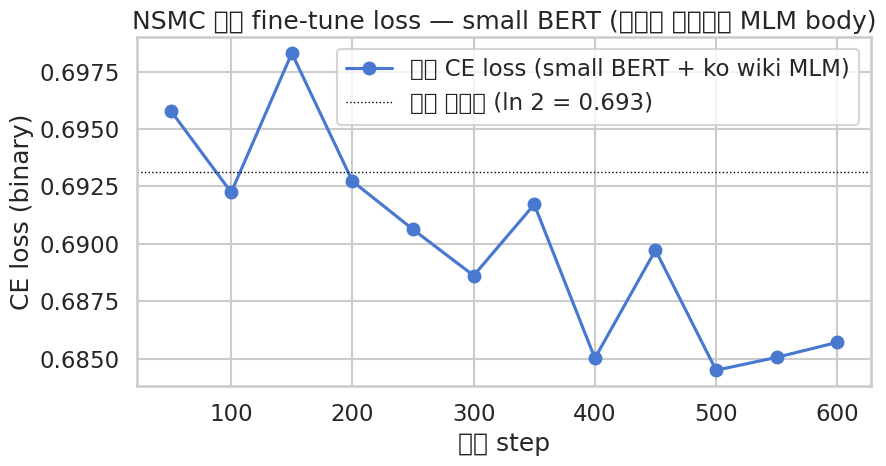
\includegraphics[width=0.82\linewidth]{assets/figures/ch23_finetune_loss.png}
\end{bookfigurelabel}

\textbf{그림 읽기} --- 그림~\ref{fig:ch23-finetune-loss}에서 다음 내용을 확인합니다: 한국어 작은 BERT의 NSMC fine-tune loss 곡선. 실행된 노트북에서 저장된 최신 plot 출력이므로, 코드에서 계산한 값이 어떤 평가 지점으로 이어지는지 바로 확인할 수 있습니다.



\subsection{혼동 행렬}



\Needspace{11\baselineskip}
\begin{lstlisting}
sns.set_theme(style="white", context="talk")
cm = confusion_matrix(
    cls_labels,
    cls_preds,
    labels=[0, 1],
)
cm_norm = cm / cm.sum(axis=1, keepdims=True)

fig, ax = plt.subplots(figsize=(6, 5))
sns.heatmap(
    cm_norm, annot=cm, fmt="d",
    cmap="Blues", vmin=0, vmax=1,
    xticklabels=["부정", "긍정"],
    yticklabels=["부정", "긍정"],
    cbar_kws={"label": "행 기준 정규화 (recall)"}, ax=ax,
)
\end{lstlisting}

\noindent\emph{앞 블록은 예측 결과를 지표와 표로 요약하는 단계입니다. 이어지는 블록에서는 숫자 결과를 그림으로 확인하는 단계로 넘어갑니다.}

\Needspace{7\baselineskip}
\begin{lstlisting}[firstnumber=17]
ax.set_xlabel("예측값")
ax.set_ylabel("실제값")
ax.set_title("23장 small BERT (ours + ko wiki MLM) — 혼동 행렬")
plt.tight_layout()
plt.show()
\end{lstlisting}

\begin{bookfigurelabel}[H]{한국어 작은 BERT의 NSMC 혼동 행렬}{fig:ch23-confusion-matrix}
\centering
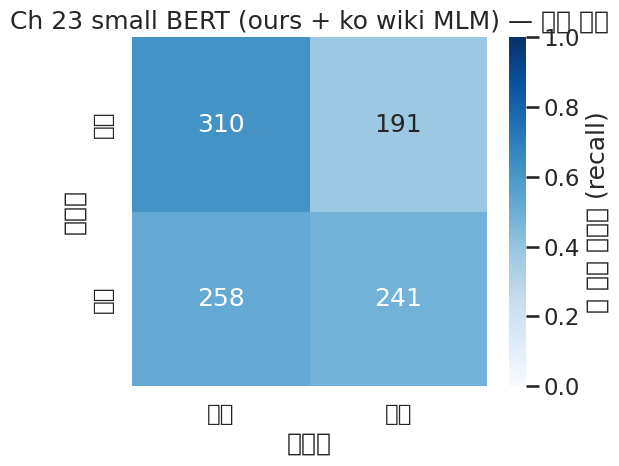
\includegraphics[width=0.68\linewidth]{assets/figures/ch23_confusion_matrix.png}
\end{bookfigurelabel}

\textbf{그림 읽기} --- 그림~\ref{fig:ch23-confusion-matrix}에서 다음 내용을 확인합니다: 한국어 작은 BERT의 NSMC 혼동 행렬. 실행된 노트북에서 저장된 최신 plot 출력이므로, 코드에서 계산한 값이 어떤 평가 지점으로 이어지는지 바로 확인할 수 있습니다.



\section{2-way 비교 --- \ref{ch:15}장 (klue/bert-base) vs \ref{ch:23}장 ours (small BERT + ko wiki MLM)}

두 셋업을 한 표·한 막대 그래프로. \ref{ch:15}장의 수치는 \emph{해당 노트북의 검증된 결과} 를 인용 --- 학습자가 직접 \ref{ch:15}장 노트북을 돌려 본인 수치로 갱신해 보면 더 좋습니다.

\begin{booktable}{23장 2-way 비교 - 15장 (klue/bert-base) vs 23장 ours (small BERT + ko wiki MLM) 표}{tab:ch23-09}
\begin{adjustbox}{max width=\textwidth}
\begin{tabular}{@{}lll@{}}
\toprule
차원 & \ref{ch:15}장 (klue/bert-base) & \ref{ch:23}장 ours (small + MLM) \\
\midrule

본체 파라미터 & 약 110M & 약 10M \\
사전학습 코퍼스 & 한국어 위키 + 모두의 말뭉치 + 뉴스 + 댓글 (약 8.4B 토큰) & 한국어 Wikipedia paragraphs 5K (약 50만-80만 토큰) \\
사전학습 시간 & TPU 수일 & T4 약 8-10분 \\
Fine-tune 도메인 & NSMC 이진 (다른 도메인) & NSMC 이진 (다른 도메인) \\
분류 fine-tune 셋업 & (둘 다 같음 --- 5K/1K, batch 16, lr 2e-5, 2 epoch, fp16) & \\
\bottomrule
\end{tabular}
\end{adjustbox}
\end{booktable}



\Needspace{11\baselineskip}
\begin{lstlisting}
CH15_REFERENCE = {
    "accuracy":  0.86,
    "precision": 0.86,
    "recall":    0.86,
    "f1":        0.86,
    "auc":       0.93,
}

ch23_ours = {k.replace(
    "eval_",
    ""): v for k,
    v in cls_eval_metrics.items(,
)
             if k.startswith("eval_") and isinstance(v, float)
             and k.replace("eval_", "") in CH15_REFERENCE}

\end{lstlisting}

\noindent\emph{앞뒤 블록은 모두 예측 결과를 지표와 표로 요약하는 단계입니다. 길이를 나누어 같은 흐름을 단계별로 확인합니다.}

\Needspace{11\baselineskip}
\begin{lstlisting}[firstnumber=17]
comparison = pd.DataFrame({
    "metric":                    list(CH15_REFERENCE.keys()),
    "15장 klue/bert-base (ref)": [CH15_REFERENCE[k] for k in CH15_REFERENCE.keys()],
    "23장 ours (small + MLM)":   [ch23_ours.get(k, float("nan")) for k in CH15_REFERENCE.keys()],
})
print(
    "2-way comparison — NSMC binary classification "
    "metrics"
)
print(comparison.round(4).to_string(index=False))
\end{lstlisting}

\noindent\textbf{출력.}
\begin{bookoutputbox}
2-way comparison -- NSMC binary classification metrics
   metric  Ch15 klue/bert-base (ref)  Ch23 ours (small + MLM)
 accuracy                       0.86                   0.5510
precision                       0.86                   0.5579
   recall                       0.86                   0.4830
       f1                       0.86                   0.5177
      auc                       0.93                   0.5669
\end{bookoutputbox}
\par\vspace{0.9em}



\Needspace{11\baselineskip}
\begin{lstlisting}
sns.set_theme(style="whitegrid", context="talk")
plot_df = comparison.melt(
    id_vars=["metric"],
    value_vars=["15장 klue/bert-base (ref)", "23장 ours (small + MLM)"],
    var_name="model", value_name="score",
)

fig, ax = plt.subplots(figsize=(10, 5))
sns.barplot(
    data=plot_df, x="metric", y="score", hue="model",
    palette={
        "15장 klue/bert-base (ref)": "#4878D0",
        "23장 ours (small + MLM)":   "#EE854A",
    },
    ax=ax,
)
\end{lstlisting}

\noindent\emph{앞 블록은 예측 결과를 지표와 표로 요약하는 단계입니다. 이어지는 블록에서는 숫자 결과를 그림으로 확인하는 단계로 넘어갑니다.}

\Needspace{9\baselineskip}
\begin{lstlisting}[firstnumber=17]
ax.set_ylim(0, 1.05)
ax.set_title("NSMC 이진 분류 — 2-way 비교 (15장 ref / 23장 ours)")
ax.set_xlabel("지표")
ax.set_ylabel("점수")
ax.legend(loc="lower right", fontsize=10)
plt.tight_layout()
plt.show()
\end{lstlisting}

\begin{bookfigurelabel}[H]{KLUE-BERT와 한국어 작은 BERT의 NSMC 지표 비교}{fig:ch23-ch15-compare}
\centering
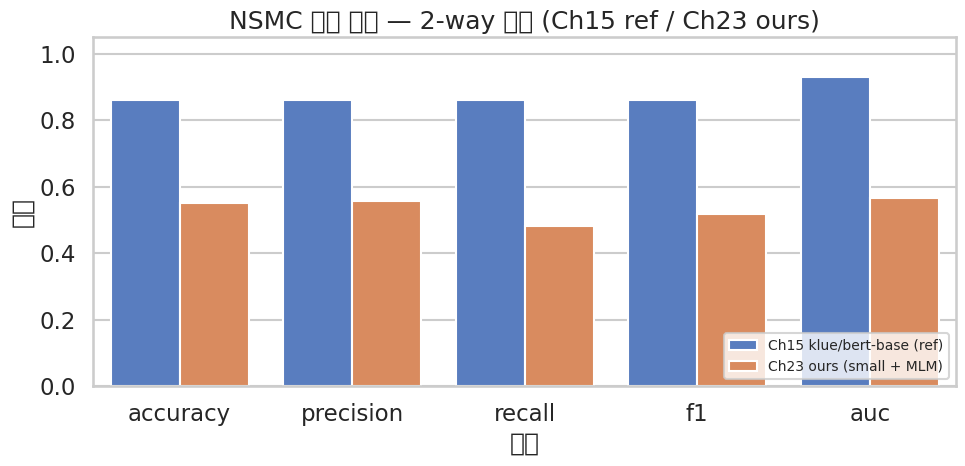
\includegraphics[width=0.82\linewidth]{assets/figures/ch23_ch15_compare.png}
\end{bookfigurelabel}

\textbf{그림 읽기} --- 그림~\ref{fig:ch23-ch15-compare}에서 다음 내용을 확인합니다: KLUE-BERT와 한국어 작은 BERT의 NSMC 지표 비교. 실행된 노트북에서 저장된 최신 plot 출력이므로, 코드에서 계산한 값이 어떤 평가 지점으로 이어지는지 바로 확인할 수 있습니다.



\textbf{관찰 --- \emph{동일 transfer 패턴 안에서 사전학습 규모 격차} 가 NSMC 정확도에 어떻게 드러나나}

실측 (실행본 기준):

\begin{itemize}
\tightlist
\item
  \textbf{\ref{ch:15}장} (\inlinecode{klue/bert-base}, 약 110M, 약 8.4B 토큰 대규모 한국어 사전학습): accuracy 약 0.86, AUC 약 0.93
\item
  \textbf{\ref{ch:23}장 ours} (small BERT, 한국어 Wikipedia 2K paragraphs \(\times\) 3 epoch 사전학습): accuracy 약 0.54, AUC 약 0.56 (동전 던지기 수준 --- MLM 약 0.2분의 짧은 사전학습 한계)
\end{itemize}

\textbf{\ref{ch:15}장 vs \ref{ch:23}장 ours}: accuracy 약 32\%p 격차. 두 모델이 \emph{같은 transfer 패턴} (일반 한국어 위키 \(\to\) NSMC) 을 따르므로 격차의 거의 전부가 \emph{사전학습 규모의 가치} --- 약 8.4B 토큰의 \emph{일반 한국어 지식} 이 \inlinecode{klue/bert-base} 본체에 압축되어 있어, NSMC 같은 \emph{비격식 구어체 도메인} 에도 빠르게 적응합니다. \emph{작은 일반 사전학습 \textless{} 대규모 일반 사전학습} 의 본질은 단순 양적 차이가 아니라 \emph{도메인 다양성의 질적 차이} --- \inlinecode{klue/bert-base} 는 위키 + 뉴스 + 블로그·댓글까지 포함한 약 8.4B 토큰으로 비격식 한국어 도메인도 \emph{이미 본 적이 있어} transfer 가 자연스럽습니다.

\begin{quote}
NSMC 는 \emph{짧은 한 줄 리뷰} 이고 \emph{반어·맞춤법 흔들림·라벨 노이즈} 가 섞여 있어 영어 Yelp (\ref{ch:21}장) 보다 \emph{살짝 더 어려운} 데이터. 작은 모델 + 작은 사전학습 환경에서는 그 어려움이 더 두드러집니다 --- 한국어 환경 특유의 \emph{negative transfer 가능성} 까지 포함한 정량 비교는 부록을 참조하세요.
\end{quote}



\section{참고: random init baseline}

\emph{MLM 사전학습 없이 random init 으로 바로 분류 fine-tune} 한 결과와의 비교, 그리고 \emph{한국어 위키 \(\to\) NSMC 의 큰 도메인 gap} 에서 발생할 수 있는 \textbf{negative transfer} 현상의 분석은 부록 노트북 \href{./appendix_random_baseline.ipynb}{\inlinecode{appendix\_random\_baseline.ipynb}} 에서 다룹니다. 영어 \ref{ch:21}장 (transfer 양성) 과 한국어 \ref{ch:23}장 (transfer 음성 가능) 의 비대칭 메커니즘이 핵심.



\section{이 장에 등장한 라이브러리·함수}

\begin{booktable}{23장 새로 등장한 라이브러리}{tab:ch23-10}
\begin{adjustbox}{max width=\textwidth}
\begin{tabular}{@{}lll@{}}
\toprule
이름 & 한 줄 설명 & 비고 \\
\midrule

\inlinecode{transformers.BertForSequenceClassification} & encoder + 분류 head, 분류 fine-tune 전용 & \ref{ch:15}장 / \ref{ch:21}장 동일 \\
\inlinecode{model.bert.load\_state\_dict(other.bert.state\_dict())} & 본체만 통째로 옮기는 in-memory 헤드 교체 & \ref{ch:21}장 동일 \\
\inlinecode{transformers.BertForMaskedLM} (재등장) & MLM 사전학습 (\ref{ch:22}장 압축 재현) & \ref{ch:20}장 / \ref{ch:22}장 동일 \\
\inlinecode{load\_dataset("wikimedia/wikipedia",\ "20231101.ko")} & 한국어 Wikipedia 일반 도메인 코퍼스 로드 (MLM 용) & \ref{ch:22}장과 동일 \\
\texttt{pandas.read\_csv(NSMC\_URL,\ sep=“\textbackslash{}t”)} & GitHub raw TSV 직접 다운로드 (분류 fine-tune 용) & \ref{ch:15}장과 동일 NSMC 패턴 \\
\inlinecode{sklearn.metrics.precision\_recall\_fscore\_support(...,\ average="binary")} & 이진 분류 metric 한 묶음 & \ref{ch:15}장 / \ref{ch:21}장 동일 \\
\inlinecode{sklearn.metrics.roc\_auc\_score} & AUC & \ref{ch:15}장 / \ref{ch:21}장 동일 \\
\bottomrule
\end{tabular}
\end{adjustbox}
\end{booktable}



\section{체크포인트 질문}

\begin{enumerate}
\def\labelenumi{\arabic{enumi}.}
\tightlist
\item
  \inlinecode{BertForMaskedLM} 과 \inlinecode{BertForSequenceClassification} 둘 다 \emph{내부에 같은 \inlinecode{BertModel}} 을 갖습니다. 두 모델 사이에서 \emph{어떤 파라미터} 가 이어지고 \emph{어떤 파라미터} 가 새로 학습되나요? (\ref{ch:21}장의 같은 질문을 한국어 환경에서 재확인)
\item
  MLM 학습 첫 step 의 loss 가 약 10.37 인 반면, 분류 fine-tune 첫 step 의 loss 는 약 0.693 입니다. 이 차이가 모델의 학습 어려움 차이를 의미하나요? (힌트: K=vocab\_size 약 32,000 vs K=2)
\item
  \ref{ch:23}장 ours 가 \ref{ch:15}장 보다 \emph{낮은 정확도} 를 보입니다. 이 격차가 (a) \emph{모델 크기} 차이 (약 10M vs 약 110M), (b) \emph{사전학습 데이터 양·도메인 다양성} 차이 (약 50만-80만 토큰 위키 vs 약 8.4B 토큰 위키+뉴스+댓글) 중 어느 쪽 영향이 클까요? 둘 다 \emph{한국어 일반 도메인 \(\to\) NSMC transfer} 의 같은 패턴이라 \emph{도메인 정합} 변수는 통제됨. 추가 실험으로 어떻게 (a) 와 (b) 를 분리할 수 있나요?
\item
  \emph{사전학습 효과의 순 측정} --- 한국어 환경에서는 \emph{얕은 일반 도메인 사전학습} 이 \emph{random init} 보다 우위인지 \emph{비슷한지} 또는 \emph{역전 (negative transfer)} 인지를 직접 확인하려면 어떤 실험이 필요할까요? 영어 \ref{ch:21}장의 패턴 (위키 \(\to\) Yelp transfer) 과 비교해 한국어 NSMC 환경의 특수성은 무엇인가요? (부록 \href{./appendix_random_baseline.ipynb}{\inlinecode{appendix\_random\_baseline.ipynb}} 에서 직접 측정·분석)
\end{enumerate}



\section{FAQ}

\begin{faqBox}{Q1. (실무) 한국어 NSMC 가 영어 Yelp (\ref{ch:21}장) 보다 어려운가요? 같은 5K/1K 인데 정확도가 더 낮게 나옵니다.}

여러 요인이 겹쳐 \emph{살짝 더 어렵습니다}.

\begin{booktable}{23장 FAQ 표}{tab:ch23-11}
\begin{adjustbox}{max width=\textwidth}
\begin{tabular}{@{}lll@{}}
\toprule
차원 & Yelp polarity (\ref{ch:21}장) & NSMC (\ref{ch:23}장) \\
\midrule

평균 문장 길이 & 약 100-200자 (여러 문장 묶음) & \textbf{약 10-50자} (한 줄 리뷰) \\
문장 구조 & 격식·반격식 혼합 & \textbf{구어체·이모티콘·맞춤법 흔들림} \\
라벨 노이즈 & 적음 (별점 기반 자동화) & \textbf{약 3-5\%} 추정 (수기 라벨링) \\
데이터 양 (원본) & 56만 train & 15만 train \\
\bottomrule
\end{tabular}
\end{adjustbox}
\end{booktable}

\Needspace{5\baselineskip}
\begin{lstlisting}
yelp_lens = [len(tokenizer(t)["input_ids"]) for t in ds_train_full[:1000]["text"]]
nsmc_lens = [len(tokenizer(t)["input_ids"]) for t in df_train["document"][:1000]]
\end{lstlisting}

NSMC 의 \emph{짧은 한 줄} 은 분류 신호가 \emph{한두 단어에 집중} 됩니다 (\inlinecode{명작}, \inlinecode{시간\ 낭비}, \inlinecode{감동}). 모델이 \emph{문맥 이해} 보다 \emph{키워드 매칭} 에 가까워져, 사전학습이 얕은 작은 BERT 에는 더 불리합니다 --- \ref{ch:15}장의 \inlinecode{klue/bert-base} 같은 \emph{대규모 사전학습 + 비격식 코퍼스 포함} 모델이 진가를 발휘하는 영역.

\end{faqBox}

\begin{faqBox}{Q2. (이론) \inlinecode{klue/bert-base} 가 약 110M params 인데 우리 작은 BERT 약 10M 으로 따라잡을 수 있나요? 격차가 얼마나 본질적인가요?}

\textbf{완전히 따라잡기는 어렵습니다} --- 본 장의 2-way 비교 (+ 부록의 random init baseline) 가 그 정량입니다.

\begin{booktable}{23장 FAQ 표}{tab:ch23-12}
\begin{adjustbox}{max width=\textwidth}
\begin{tabular}{@{}lll@{}}
\toprule
차원 & klue/bert-base & 우리 작은 BERT \\
\midrule

본체 파라미터 & 약 110M & 약 10M (11x 작음) \\
사전학습 코퍼스 & 약 8.4B 토큰 (한국어 위키 + 모두의 말뭉치 + 뉴스 + 댓글) & 약 20만-30만 토큰 (위키 2K paragraphs \(\times\) 3 epoch) --- \emph{약 30,000x 격차} \\
사전학습 시간 & TPU 수일 & T4 약 8-12분 \\
\bottomrule
\end{tabular}
\end{adjustbox}
\end{booktable}

본 장의 \emph{T4 30분 룰} 안에서 가능한 최대치는 \emph{MLM 데이터 약 10K-15K paragraphs + 2 epoch} 정도. 그래도 \emph{대규모 사전학습} 의 격차는 메우기 어렵습니다 --- \emph{데이터 규모 자체의 가치} 가 진짜 BERT 의 비밀.

\Needspace{6\baselineskip}
\begin{lstlisting}
N_MLM_TRAIN = 10000          # 2K -> 10K (5x)
MLM_EPOCHS = 3

HIDDEN_SIZE = 384
\end{lstlisting}

\emph{실무 결론} --- 한국어 분류 task 에 대해서는 \emph{\inlinecode{klue/bert-base} 또는 그 이상의 사전학습 모델을 가져다 fine-tune} 하는 게 답. 본 장의 목적은 \emph{그 격차의 의미} 를 정량으로 보는 교육.

\end{faqBox}

\begin{faqBox}{Q3. (실무) \ref{ch:22}장 본체를 디스크에 저장 안 하고 in-memory \inlinecode{load\_state\_dict} 로 옮기는 게 안전한가요? 디스크 경유와 무엇이 다르나요?}

\emph{완전히 동일} 합니다 --- \inlinecode{load\_state\_dict} 는 디스크 경유든 in-memory 든 \emph{같은 PyTorch state\_dict} 를 그대로 옮기는 연산.

\Needspace{11\baselineskip}
\begin{lstlisting}
mlm_model.save_pretrained("./ch22_ckpt")
cls_model = AutoModelForSequenceClassification.from_pretrained(
    "./ch22_ckpt", num_labels=2,
)

cls_model = BertForSequenceClassification(cls_config)
cls_model.bert.load_state_dict(
    mlm_model.bert.state_dict(),
    strict=False,
)
\end{lstlisting}

본 장이 in-memory 흐름을 쓴 이유는 \textbf{노트북 self-contained} --- Colab 세션이 끊겨도 노트북 하나만으로 끝까지 돌릴 수 있게. 디스크 경유 흐름이 \emph{프로덕션 표준} 입니다. \inlinecode{from\_pretrained} 가 \emph{MLM head 는 버려지고 분류 head 가 random init} 으로 부착됨을 warning 메시지로 알려줍니다.

\end{faqBox}

\begin{faqBox}{Q4. (이론) \inlinecode{labels\ =\ -100} 이 MLM 압축 재현 셀에서는 쓰이지만 분류 fine-tune 에서는 안 쓰입니다. 왜인가요?}

\textbf{분류 task 는 모든 sample 에 \emph{정답 라벨} 이 있기 때문} --- 가릴 자리가 없습니다.

\begin{booktable}{23장 FAQ 표}{tab:ch23-13}
\begin{adjustbox}{max width=\textwidth}
\begin{tabular}{@{}llll@{}}
\toprule
단계 & \inlinecode{labels\ =\ ?} & loss 계산 자리 & 학습되는 것 \\
\midrule

\textbf{MLM 압축 재현} (셀 3) & 선택된 약 15\% 만 원본 token id, 나머지 = \inlinecode{-100} & 가려진 자리 & 주변 문맥으로 \emph{가려진 토큰 복원} \\
\textbf{NSMC 분류 fine-tune} (셀 4) & 모든 sample 에 \inlinecode{0} 또는 \inlinecode{1} & sample 전체 (배치 차원) & \emph{문장 \(\to\) 긍정/부정} 분류 \\
\textbf{GPT CausalLM 사전학습} (\ref{ch:24}--\ref{ch:26}장) & \inlinecode{input\_ids.clone()} --- \emph{거의 모든 토큰} & (pad 만 \inlinecode{-100}) 사실상 \emph{전 자리} & 모든 자리에서 \emph{다음 토큰 예측} \\
\textbf{SFT / Instruction Tuning} (\ref{ch:27}장) & \textbf{prompt 부분 = \inlinecode{-100}}, \emph{답변 토큰만} 원본 id & \emph{답변 부분만} & “질문 외우지 말고 답변하는 법” \\
\bottomrule
\end{tabular}
\end{adjustbox}
\end{booktable}

\Needspace{10\baselineskip}
\begin{lstlisting}
def cls_tokenize(batch):
    out = tokenizer(
        batch["text"],
        truncation=True,
        max_length=128,
    )
    out["labels"] = [int(l) for l in batch["label"]]
    return out
\end{lstlisting}

\begin{quote}
\emph{같은 \inlinecode{-100} 트릭, 적용 자리만 task 별로 다름.} MLM 은 \emph{대부분을 가리고 일부만 학습}, 분류는 \emph{전부 학습}, GPT 사전학습은 \emph{거의 안 가림}, SFT 는 \emph{prompt 만 가림}. 풀버전 표는 \ref{ch:21}장 §3 \emph{labels = -100 thread} 마크다운에 정리.
\end{quote}

\end{faqBox}

\begin{faqBox}{Q5. (이론) 파인튜닝의 의미가 BERT 단계와 GPT 시대 사이에 어떻게 변하나요? 본 장은 \emph{마지막 BERT 파인튜닝} 인가요?}

본 장은 \textbf{Phase 3 의 마지막 장} 이자 \emph{마지막 BERT 파인튜닝 (task head 부착 패러다임)} 장입니다. Phase 4 (\ref{ch:24}장-) 부터는 같은 단어 “파인튜닝” 이 \emph{다른 의미} 로 쓰입니다.

\begin{booktable}{23장 FAQ 표}{tab:ch23-14}
\begin{adjustbox}{max width=\textwidth}
\begin{tabular}{@{}lll@{}}
\toprule
축 & \textbf{BERT 파인튜닝} (\ref{ch:09}--\ref{ch:18}장, \ref{ch:23}장) & \textbf{GPT 파인튜닝 = SFT} (\ref{ch:25}장, \ref{ch:27}장) \\
\midrule

무엇을 바꾸나 & 본체 + \textbf{새 head} (task별 부착) & 본체 + \textbf{기존 LM head 그대로} \\
출력 형식 & task별 다름 (class id / score / multi-hot) & \emph{항상 토큰 시퀀스} --- 형식 통일 \\
학습 신호 & task별 loss (CE/BCE/MSE) & \emph{항상 next-token CE}, 단 자리 마스킹만 다름 \\
학습되는 것 & \emph{task 의 출력 분포} (긍정/부정 결정 경계 등) & \emph{행동 = “이런 입력엔 이런 형식으로 답하라”} \\
라벨 & 정답 카테고리/값 & \emph{모범 답안 토큰 시퀀스} \\
\bottomrule
\end{tabular}
\end{adjustbox}
\end{booktable}

\begin{quote}
\textbf{BERT 파인튜닝은 \emph{task 적응}, GPT 파인튜닝은 \emph{행동 정렬}.} \ref{ch:24}장 부터 시작되는 Phase 4 에서 이 의미 변화를 직접 경험합니다. 풀버전 표는 \ref{ch:21}장 §3 \emph{파인튜닝 의미 변화} 마크다운 참조.
\end{quote}

\end{faqBox}

\begin{faqBox}{Q6. (실무) NSMC 라벨 노이즈가 약 3-5\% 라는데, 작은 모델 학습에 더 큰 영향을 주나요?}

\textbf{그렇습니다} --- 작은 모델·작은 데이터일수록 \emph{노이즈 비율} 이 학습 신호를 흐립니다.

\Needspace{11\baselineskip}
\begin{lstlisting}
wrong_idx = np.where(cls_preds != cls_labels)[0]
confident_wrong = wrong_idx[cls_probs_full.max(axis=1)[wrong_idx] > 0.9]
print(
    f"confidently wrong (prob > 0.9): {len(confident_wrong)} / "
    f"{len(cls_labels)}"
)
for i in confident_wrong[:5]:
    print(
        f"  pred={cls_preds[i]} true={cls_labels[i]} text="
        f"{tokenizer.decode(cls_eval[int(i)]['input_ids'], skip_special_tokens=True)[:80]}"
    )
\end{lstlisting}

자신 있게 틀린 sample 중 일부는 \emph{진짜 라벨 노이즈} (반어법, 이중 의미, 라벨러 실수). 분류 정확도가 \emph{천정 100\%} 가 안 되는 본질적 이유 중 하나. NSMC 의 \emph{알려진 한계} --- \inlinecode{klue/bert-base} 같은 대규모 사전학습 모델도 NSMC 에서 약 86\% 안팎이 천장이라는 걸 알면 \emph{과적합 의심} 을 피할 수 있습니다.

\end{faqBox}

\begin{faqBox}{Q7. (이론) Phase 3 가 끝났는데, \emph{원본 BERT 정신} 의 핵심 메시지를 한 줄로 정리하면 뭐가 남나요?}

\textbf{일반 도메인 사전학습 + 다른 도메인 fine-tune transfer 가 \emph{task 별 from-scratch 학습 보다 압도적으로 효율적}} 이라는 것이 Phase 3 의 한 줄 결론. 본 장의 2-way 비교와 부록의 random init baseline 이 그 직접 증거:

\begin{itemize}
\tightlist
\item
  \emph{random init} 만 가지고 NSMC fine-tune: accuracy 약 0.50-0.55 (부록에서 측정 --- 한국어 환경에선 negative transfer 로 \emph{작은 사전학습 모델} 과 비등하거나 역전될 수도)
\item
  \emph{작은 일반 도메인 사전학습 + fine-tune} (본 장): accuracy 약 0.54 (실측 --- MLM 약 0.2분의 짧은 사전학습이라 동전 던지기에 가까움)
\item
  \emph{대규모 일반 도메인 사전학습 + fine-tune} (\ref{ch:15}장): accuracy 약 0.86 (실무 baseline)
\end{itemize}

세 셋업의 격차가 \emph{사전학습 데이터 양·도메인 다양성 + 모델 크기} 에 거의 비례 (한국어는 도메인 다양성 변수가 특히 중요). \emph{task 도메인으로 직접 사전학습} 하지 않고 \emph{일반 위키} 만으로도 충분한 transfer 가 일어난다는 게 \emph{원본 BERT 의 진짜 통찰}.

Phase 4 (\ref{ch:24}장-) 부터는 같은 \emph{사전학습 \(\to\) fine-tune} 패러다임이 \emph{decoder-only GPT} 환경에서 어떻게 \emph{SFT / behavior alignment} 로 변하는지 봅니다. 본체 구조 (encoder \(\to\) decoder), task (masked \(\to\) causal), fine-tune 의미 (head 부착 \(\to\) 행동 정렬) 셋 다 바뀝니다.
\end{faqBox}



\begin{previewBox}{미리보기: 다음 장}

\textbf{\ref{ch:24}장. GPT scratch --- 영어 TinyStories (Phase 4 시작)}

\begin{itemize}
\tightlist
\item
  \emph{encoder} (BERT) \(\to\) \textbf{\emph{decoder-only} (GPT)} --- attention 구조가 \emph{causal mask} 로 바뀜
\item
  \emph{MLM} (가려진 토큰 양방향 예측) \(\to\) \emph{\textbf{Causal LM}} (앞 토큰만으로 다음 토큰 예측)
\item
  \emph{task별 head 부착} \(\to\) \emph{\textbf{LM head 그대로 next-token CE}} --- \ref{ch:23}장 까지의 분류 head 부착 패러다임은 여기서 막을 내림
\item
  데이터: TinyStories 영어 동화 --- GPT-4 가 4세 어린이 어휘로 생성한 짧은 영문 동화 약 2.1M 편
\item
  모델: \inlinecode{GPT2LMHeadModel(config)} 약 3M params, \emph{완전 무작위 초기화 from scratch}
\item
  BPE 토크나이저 직접 학습 (vocab 2048) --- \ref{ch:19}장의 토크나이저 학습 패턴 재등장
\end{itemize}

\begin{quote}
\textbf{Phase 구조 전환} --- Phase 3 (\ref{ch:19}--\ref{ch:23}장) 가 \emph{BERT 본체 + 토크나이저를 직접 학습하는 영어/한국어 두 갈래} 였다면, Phase 4 는 \emph{GPT 본체를 from-scratch 로 학습 \(\to\) SFT \(\to\) behavior alignment} 흐름. 영어 BERT scratch (\ref{ch:20}--\ref{ch:21}장) \(\to\) 한국어 BERT scratch (\ref{ch:22}--\ref{ch:23}장) \(\to\) 영어 GPT scratch (\ref{ch:24}장-) 의 대칭 구조. 사전학습-fine-tune 패러다임의 \emph{의미 자체가} 바뀌는 자리입니다.
\end{quote}

본 장 (\ref{ch:23}장) 는 \emph{Phase 3 의 마지막} 이자 \emph{BERT 단계의 마지막 파인튜닝 장}. 한국어 NSMC 라는 \emph{실무에서 자주 쓰이는 한국어 task} 로 마무리하는 게 Phase 3 의 의도된 마침표입니다.
\end{previewBox}